%# -*- coding:utf-8 -*-
\documentclass[12pt,aspectratio=169,mathserif]{beamer}		
%设置为 Beamer 文档类型，设置字体为 10pt，长宽比为16:9，数学字体为 serif 风格

%%%%-----导入宏包-----%%%%
\usepackage{zju}			%导入 zju 模板宏包
%\usepackage{ctex}			%导入 ctex 宏包，添加中文支持
\usepackage{amsmath,amsfonts,amssymb,bm}   %导入数学公式所需宏包
\usepackage{color}			 %字体颜色支持
\usepackage{graphicx,hyperref,url}
\usepackage{metalogo}	% 非必须
%% 上文引用的包可按实际情况自行增删
%%%%%%%%%%%%%%%%%%
\usepackage{fontspec}
\usepackage{xeCJK}
% \setCJKmainfont{Source Han Sans SC}
\usepackage{tcolorbox}
\beamertemplateballitem		%设置 Beamer 主题

%%%%------------------------%%%%%
\catcode`\。=\active         %或者=13
\newcommand{。}{．}				
%将正文中的“。”号转换为“.”。中文标点国家规范建议科技文献中的句号用圆点替代
%%%%%%%%%%%%%%%%%%%%%

%%%%----首页信息设置----%%%%
\title[Distance Metric Learning for LMNN Classification]{Distance Metric Learning \\ for Large Margin Nearest Neighbor Classification}			
%%%%----标题设置


\author[Zhetao Wang, Xiang Ye, Jiayan He, Zhouyue Qian]{
  王哲涛\ 叶翔\ 贺嘉言\ 钱周越 \\\medskip}
%%%%----个人信息设置
  
\institute[IOPP]{
  数学科学学院 \\ 
  浙江大学}
%%%%----机构信息

\date[May. 6th, 2025]{
  2025年5月6日}
%%%%----日期信息
  
\begin{document}

\begin{frame}
	\titlepage
\end{frame}				%生成标题页

\section{Outline}
\begin{frame}
	\frametitle{Outline}
	\tableofcontents
\end{frame}				%生成提纲页

\section{Introduction}

\begin{frame}
    \centering
    \Huge \insertsection % 插入章节标题
\end{frame}

\begin{frame}
\frametitle{The Problem}
\begin{itemize}
    \item k-Nearest Neighbor (kNN) Classification
    \begin{itemize}
      \item Simple, effective rule: Classify by majority label of $k$ closest training examples.
      \item Performance depends crucially on the distance metric used.
    \end{itemize}
    \item Default: Euclidean Distance
    \begin{itemize}
      \item Ignores statistical regularities in data.
      \item Example: Same metric for face age vs. gender classification is suboptimal.
    \end{itemize}
	\item Motivation: Improve kNN accuracy by learning an appropriate distance metric from labeled data.
	\begin{itemize}
	\item Previous work showed simple linear transformations help.
	\item We aim to learn a \textbf{Mahalanobis distance metric}.
	\end{itemize}
\end{itemize}
\end{frame}

\begin{frame}
\frametitle{Our Approach - LMNN}
\begin{itemize}
    \item Intuition: A kNN classifier is accurate if:
    \begin{itemize}
      \item An example's $k$-nearest neighbors belong to the same class.
      \item Examples from different classes are separated by a large margin.
    \end{itemize}
    \item LMNN aims to learn a linear transformation (Mahalanobis metric) that achieves these properties.
    \item Achieved by minimizing a loss function:
    \begin{itemize}
      \item Penalizes large distances between desired neighbors.
      \item Penalizes small distances between differently labeled examples (using a hinge loss for a margin).
    \end{itemize}
    \item This yields a convex optimization problem.
  \end{itemize}
\end{frame}

\section{Background}

\begin{frame}
    \centering
    \Huge \insertsection % 插入章节标题
\end{frame}

\begin{frame}
\frametitle{Distance Metrics}
\begin{itemize}
	\item Definition: A mapping $D: \mathcal{X} \times \mathcal{X} \rightarrow \mathfrak{R}_{0}^{+}$ is a metric if it satisfies:
	\begin{enumerate}
	\item Triangular inequality: $D(\vec{x}_{i}, \vec{x}_{j}) + D(\vec{x}_{j}, \vec{x}_{k}) \geq D(\vec{x}_{i}, \vec{x}_{k})$
	\item Non-negativity: $D(\vec{x}_{i}, \vec{x}_{j}) \geq 0$
	\item Symmetry: $D(\vec{x}_{i}, \vec{x}_{j}) = D(\vec{x}_{j}, \vec{x}_{i})$
	\item Distinguishability: $D(\vec{x}_{i}, \vec{x}_{j}) = 0 \Longleftrightarrow \vec{x}_{i} = \vec{x}_{j}$
	\end{enumerate}
	\item Pseudometric: Satisfies 1-3 but not necessarily 4.
\end{itemize}
\end{frame}

\begin{frame}
\frametitle{Mahalanobis Distance}
\begin{itemize}
	\item A family of metrics/pseudometrics derived from a linear transformation $\vec{x}' = \mathbf{L}\vec{x}$ followed by Euclidean distance.
	\item Squared distance:
	\[
	D_{\mathbf{L}}(\vec{x}_i, \vec{x}_j) = \|\mathbf{L}(\vec{x}_i - \vec{x}_j)\|_2^2
	\]
	\item Can be expressed in terms of a positive semidefinite matrix $\mathbf{M}$:
	\[
	\mathbf{M} = \mathbf{L}^\top \mathbf{L} \quad \implies \quad \mathcal{D}_{\mathbf{M}}(\vec{x}_i, \vec{x}_j) = (\vec{x}_i - \vec{x}_j)^\top \mathbf{M} (\vec{x}_i - \vec{x}_j)
	\]
	\item Euclidean distance is a special case when $\mathbf{M}$ is the identity matrix.
	\item Metric learning goal: Estimate $\mathbf{L}$ or $\mathbf{M}$ from labeled data $\{( \vec{x}_i, y_i )\}_{i=1}^n$.
\end{itemize}
\end{frame}

\begin{frame}
\frametitle{Review of Previous Approaches}
\begin{itemize}
	\item Broadly classified into three categories:
	\begin{enumerate}
	\item Eigenvector Methods (based on second-order statistics).
	\item Convex Optimizations (over positive semidefinite matrices).
	\item Fully Supervised Algorithms (directly optimizing kNN criteria).
	\end{enumerate}
	\item These approaches provide context and motivation for LMNN.
\end{itemize}
\end{frame}

\begin{frame}
\frametitle{Eigenvector Methods}
\textbf{Principal Component Analysis (PCA)}
\begin{itemize}
	\item Goal: Compute $\mathbf{L}$ that projects data into a variance-maximizing subspace.
	\item Method: Unsupervised. Based on input covariance matrix $\mathbf{C}$.
	\[
	\mathbf{C}=\frac{1}{n} \sum_{i=1}^{n}\left(\vec{x}_{i}-\vec{\mu}\right)^{\top}\left(\vec{x}_{i}-\vec{\mu}\right)
	\]
	\item Optimization:
	\[
	\max _{\mathbf{L}} \operatorname{Tr}\left(\mathbf{L}^{\top} \mathbf{C} \mathbf{L}\right) \text { subject to: } \mathbf{L} \mathbf{L}^{\top}=\mathbf{I}
	\]
	\item Solution: Rows of $\mathbf{L}$ are leading eigenvectors of $\mathbf{C}$.
\end{itemize}
\end{frame}

\begin{frame}
\frametitle{Eigenvector Methods}
\textbf{Linear Discriminant Analysis (LDA)}
\begin{itemize}
	\item Goal: Compute $\mathbf{L}$ that maximizes the ratio of between-class to within-class variance.
	\item Method: Supervised. Based on between-class ($\mathbf{C}_b$) and within-class ($\mathbf{C}_w$) covariance matrices.
	\begin{align*}
	\mathbf{C}_{b}  =\frac{1}{\mathcal{C}} \sum_{c=1}^{\mathcal{C}} \vec{\mu}_{c} \vec{\mu}_{c}^{\top} \quad
	\mathbf{C}_{w}  =\frac{1}{n} \sum_{c=1}^{\mathcal{C}} \sum_{i \in \Omega_{c}}\left(\vec{x}_{i}-\vec{\mu}_{c}\right)\left(\vec{x}_{i}-\vec{\mu}_{c}\right)^{\top}
	\end{align*}
	\item Optimization:
	\[
	\max _{\mathbf{L}} \operatorname{Tr}\left(\frac{\mathbf{L}^{\top} \mathbf{C}_{b} \mathbf{L}}{\mathbf{L}^{\top} \mathbf{C}_{w} \mathbf{L}}\right) \text { subject to: } \mathbf{L L}^{\top}=\mathbf{I}
	\]
	\item Solution: Rows of $\mathbf{L}$ are leading eigenvectors of $\mathbf{C}_{w}^{-1} \mathbf{C}_{b}$.
\end{itemize}
\end{frame}

\begin{frame}
\frametitle{Eigenvector Methods}
\textbf{Relevant Component Analysis (RCA)}
\begin{itemize}
	\item Goal: Compute $\mathbf{L}$ that whitens data w.r.t. averaged within-"chunklet" covariance.
	\item Method: Supervised, uses "chunklet" information (subsets of a class). $\Omega_{\ell}$ is the set of indices in chunklet $\ell$.
	\[
	\mathbf{C}_{w}=\frac{1}{n} \sum_{l=1}^{L} \sum_{i \in \Omega_{l}}\left(\vec{x}_{i}-\vec{\mu}_{l}\right)\left(\vec{x}_{i}-\vec{\mu}_{l}\right)^{\top}
	\]
	\item Linear transformation $\vec{x}_{i} \rightarrow \mathbf{L} \vec{x}_{i}$ with $\mathbf{L}=\mathbf{C}_{w}^{-1 / 2}$.
	\item Often used after PCA.
\end{itemize}
\end{frame}


\begin{frame}{Convex Optimization}
    \textbf{Mahalanobis Metric for Clustering (MMC)}
    \begin{itemize}
        \item Goal: Learn $\mathbf{M}$ for clustering, minimizing distances between similarly labeled inputs, maximizing distances between differently labeled inputs.
        \item Comparison to LDA: Similar goal, but formulated as a convex optimization over $\mathbf{M}$ instead of an eigenvalue problem for $\mathbf{L}$.
        \item Formulation: Convex optimization over $\mathbf{M}$. Uses binary association matrix $y_{ij}=1$ if $y_i=y_j$, 0 otherwise.
        \begin{tcolorbox}[title=,colframe=black,colback=white,boxrule=0.5pt, width=0.7\textwidth]
            \textbf{Maximize} $\sum_{ij}(1-y_{ij})\sqrt{\mathcal{D}_{\mathbf{M}}(\vec{x}_i,\vec{x}_j)}$ \textbf{subject to:}\\
            (1) $\sum_{ij}y_{ij}\mathcal{D}_{\mathbf{M}}(\vec{x}_i,\vec{x}_j) \leq 1$\\
            (2) $\mathbf{M} \succeq 0$.
        \end{tcolorbox}
    \end{itemize}
\end{frame}

\begin{frame}{Convex Optimization}
    \textbf{Pseudometric Online Learning Algorithm (POLA)}
    \begin{itemize}
        \item Goal: Perceptron-like online learning of $\mathbf{M}$ with an explicit margin. Shrink distances for same-label pairs, expand for different-label pairs.
        \item Comparison to LDA/MMC: Also aims to separate classes, but introduces a finite margin and can work online.
        \item Online Setting: Receives tuples $(\vec{x}_t, \vec{x}_t', y_t)$ with $y_t \in \{1, -1\}$
        \item Margin Constraint: Aims for similarly labeled pairs $\leq b-1$ distance, differently labeled pairs $\geq b+1$ distance.
        $$ y_{t}\left[b-\mathcal{D}_{\mathbf{M}}\left(\vec{x}_{t}, \vec{x}_{t}^{\prime}\right)\right] \geq 1 $$
        \item Method: Updates $\mathbf{M}$ and $b$ online using an alternating projection algorithm to correct margin violations. $\mathbf{M}$ remains PSD after updates.
    \end{itemize}
\end{frame}

\begin{frame}{Neighborhood Component Analysis (NCA)}
    \begin{itemize}
        \item Goal: Learn a Mahalanobis metric $\mathbf{M}$ (or $\mathbf{L}$) specifically to improve kNN classification accuracy.
        \item Approach: Minimize the expected leave-one-out (LOO) classification error using a \textbf{stochastic} variant of kNN.
        \item Stochastic kNN: Probability $p_{ij}$ of $\vec{x}_j$ being chosen as a reference for $\vec{x}_i$ is based on a softmax over distances $\mathcal{D}_{\mathbf{L}}(\vec{x}_i, \vec{x}_j)$:
        \[
        p_{i j}=\left\{\begin{array}{cc}
        \frac{\exp \left(-\left\|\mathbf{L} \vec{x}_{i}-\mathbf{L} \vec{x}_{j}\right\|^{2}\right)}{\sum_{k \neq i} \exp \left(-\left\|\mathbf{L} \vec{x}_{i}-\mathbf{L} \vec{x}_{k}\right\|^{2}\right)} & \text { if } i \neq j \\
        0 & \text { if } i=j .
        \end{array}\right.
        \]
        (No fixed $k$ parameter; scale of $\mathbf{L}$ controls neighborhood size).
    \end{itemize}
\end{frame}

\begin{frame}{Neighborhood Component Analysis (NCA)(cont.)} 
    \begin{itemize} 
        \item Objective: Expected LOO classification accuracy on training data. Minimizing error is maximizing expected accuracy.
        \[\mathcal{E}_{\mathrm{NCA}}=1-\frac{1}{n} \sum_{i j} p_{i j} y_{i j}\]
        \item The objective function $\mathcal{E}_{\mathrm{NCA}}$ is continuous and differentiable w.r.t. $\mathbf{L}$ (or $\mathbf{M}$), unlike deterministic kNN LOO error. This allows optimization via gradient descent.
        \item The objective function is non-convex. Optimization can get stuck in spurious local minima, results depend on initialization.
    \end{itemize}
\end{frame}
\section{Model}

\begin{frame}
    \centering
    \Huge \insertsection % 插入章节标题
\end{frame}

\begin{frame}
\frametitle{Building on Distance Metric Learning}

\begin{itemize}
	\item Goal: Learn a Mahalanobis distance metric $$\mathcal{D}_{\mathbf{M}}(\vec{x}_i, \vec{x}_j) = (\vec{x}_i - \vec{x}_j)^{\top} \mathbf{M} (\vec{x}_i - \vec{x}_j) \text{ where } \mathbf{M} \succeq 0.$$
	\item $\mathbf{M}$ is learned from labeled data.
	\item Builds on existing approaches:
	\begin{itemize}
	\item \textbf{MMC}: Formulate estimation as convex optimization ($\mathbf{M} \succeq 0$).
	\item \textbf{POLA}: Maximize classification margin.
	\item \textbf{NCA}: Specifically designed to improve $k$NN classification.
	\end{itemize}

\end{itemize}
\end{frame}

\begin{frame}
\frametitle{Intuition for Robust $k$NN}

Two simple intuitions guide the model:

\begin{enumerate}
	\item \textbf{Neighborhood Homogeneity}: Each training input $\vec{x}_i$ should share the same label $y_i$ as its $k$ nearest neighbors (in the learned metric).
	\item \textbf{Class Separation}: Training inputs with different labels should be widely separated.
	\end{enumerate}

	These are balanced by competing terms in the loss function:
	\begin{itemize}
	\item Term 1: Penalizes large distances between nearby inputs with the same label. (Pull)
	\item Term 2: Penalizes small distances between inputs with different labels. (Push)
\end{itemize}

\end{frame}

\begin{frame}
\frametitle{Key Terminology}

\begin{itemize}
	\item \textbf{Target Neighbors} ($j \rightsquigarrow i$):
	\begin{itemize}
	\item Training inputs $\vec{x}_j$ that we desire to be closest to $\vec{x}_i$.
	\item Fixed \textit{a priori} (e.g., $k$ nearest neighbors of $\vec{x}_i$ with the same class label $y_i$ using Euclidean distance).
	\end{itemize}
	\item \textbf{Importors}:
	\begin{itemize}
		\item Training inputs $\vec{x}_l$ with a different label ($y_l \neq y_i$), $\vec{x}_l$ is an importor if $\|\mathbf{L}(\vec{x}_i - \vec{x}_l)\|^2 \leq \|\mathbf{L}(\vec{x}_i - \vec{x}_j)\|^2 + 1.$
		\item Goal of learning: minimize the number of importors.
	\end{itemize}
	\item \textbf{Margin}:
	\begin{itemize}
	\item Maintain a large distance between importors and the perimeters defined by target neighbors.
	\item Improves robustness to noise.
	\end{itemize}
\end{itemize}
\end{frame}

\begin{frame}
	\frametitle{Schematic Illustration}
\begin{figure}
  \centering
  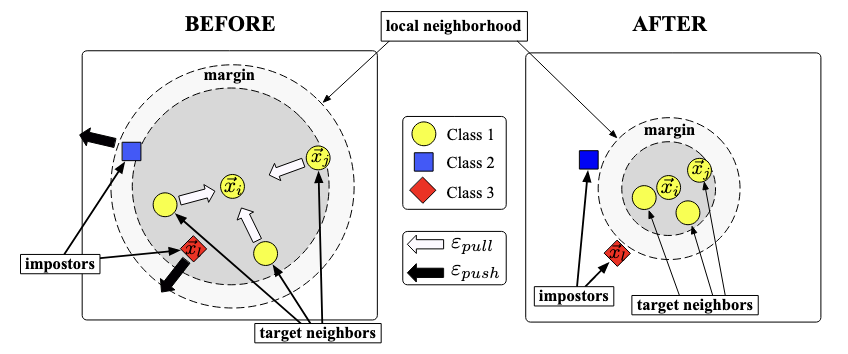
\includegraphics[width=0.8\textwidth]{res/illustration.png}
  \caption{LMNN Learning Illustration}
  \label{fig:lmnn}
\end{figure}
\end{frame}

\begin{frame}
  \frametitle{Loss Function}
  \begin{itemize}
    \item The loss function consists of two parts: $$\varepsilon(\mathbf{L})=(1-\mu) \varepsilon_{pull }(\mathbf{L})+\mu \varepsilon_{push }(\mathbf{L}),$$  where $\mu \in[0,1]$ is a balancing parameter, typically set to 0.5.
    \item $\varepsilon_{pull }(\mathbf{L})=\sum_{j \rightsquigarrow i}\left\| \mathbf{L}\left(\vec{x}_{i}-\vec{x}_{j}\right)\right\| ^{2}$ \label{eq:pull_term}, which penalizes large distances between each input and its target neighbors, attracting target neighbors closer.
    \item $\varepsilon_{push }(\mathbf{L})=\sum_{i, j \rightsquigarrow i} \sum_{l}\left(1-y_{i l}\right)\left[1+\left\| \mathbf{L}\left(\vec{x}_{i}-\vec{x}_{j}\right)\right\| ^{2}-\left\| \mathbf{L}\left(\vec{x}_{i}-\vec{x}_{l}\right)\right\| ^{2}\right]_{+}$ \label{eq:push_term}, which uses hinge loss to penalize small distances between differently-labeled samples, pushing impostors away.
\end{itemize} 
\end{frame}

\begin{frame}
\frametitle{Local vs. Global Distances}

\begin{itemize}
	\item LMNN's focus on pulling only \textit{target neighbors} (local) is a key distinction.
	\item Many previous methods (LDA, RCA, MCC) try to shrink distances between \textit{all} examples in the same class (global). 
\end{itemize}

\begin{figure}
	\centering
	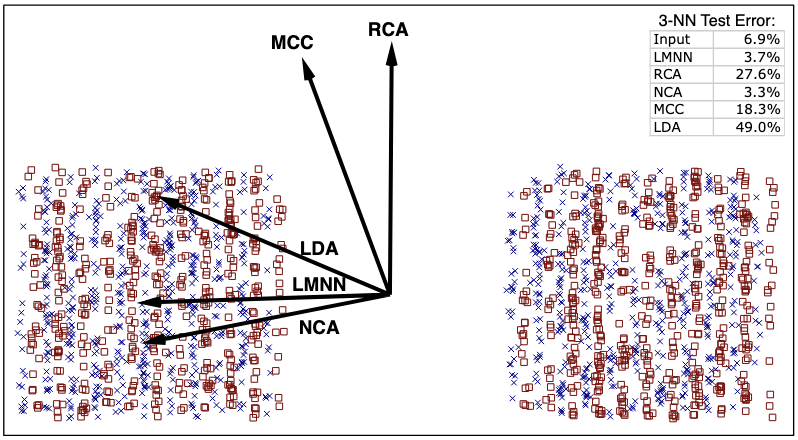
\includegraphics[width=0.5\textwidth]{res/toy_data.png}
	\vspace{-0.5em}
	\caption{Toy Data Example}
\end{figure}
\end{frame}

\begin{frame}{Convex Optimization}
    \textbf{Problem with Optimization in $\mathbf{L}$:}
    \begin{itemize}
        \item The loss function $\varepsilon(\mathbf{L})$ is \emph{not convex} in $\mathbf{L}$.
        \item Gradient descent in $\mathbf{L}$ is prone to being trapped in spurious local minima.
    \end{itemize}

    \textbf{Solution: Reformulate as Convex Optimization over $\mathbf{M}$}
    \begin{itemize}
        \item Use the variable $\mathbf{M} = \mathbf{L}^\top \mathbf{L}$, the constraint $\mathbf{M} \succeq 0$ is convex.
        \item Loss Function in terms of $\mathbf{M}$:
        \begin{align*} \varepsilon(\mathbf{M})&=(1-\mu) \sum_{i} \sum_{j \rightsquigarrow i} \mathcal{D}_{\mathbf{M}}\left(\vec{x}_{i}, \vec{x}_{j}\right)\\
        &+\mu \sum_{i} \sum_{j \rightsquigarrow i} \sum_{l}\left(1-y_{i l}\right)\left[1+\mathcal{D}_{\mathbf{M}}\left(\vec{x}_{i}, \vec{x}_{j}\right)-\mathcal{D}_{\mathbf{M}}\left(\vec{x}_{i}, \vec{x}_{l}\right)\right]_{+}. \end{align*}
    \end{itemize}
\end{frame}

\begin{frame}{Convex Optimization(cont.)}
    \textbf{Formulation as a Semidefinite Program (SDP):}
    \begin{tcolorbox}[title=LMNN SDP,colframe=black,colback=white,boxrule=0.5pt, width=\textwidth]
        \textbf{Minimize:}\\ $(1-\mu) \sum_{i, j \rightsquigarrow i}\left(\vec{x}_{i}-\vec{x}_{j}\right)^{\top} \mathbf{M}\left(\vec{x}_{i}-\vec{x}_{j}\right)+\mu \sum_{i, j \rightsquigarrow i, l}\left(1-y_{i l}\right) \xi_{i j l}$\\
        \textbf{subject to:}\\
        (1) $\left(\vec{x}_{i}-\vec{x}_{l}\right)^{\top} \mathbf{M}\left(\vec{x}_{i}-\vec{x}_{l}\right)-\left(\vec{x}_{i}-\vec{x}_{j}\right)^{\top} \mathbf{M}\left(\vec{x}_{i}-\vec{x}_{j}\right) \geq 1-\xi_{i j l}, \quad \forall i, j \rightsquigarrow i, l$\\
        (2) $\xi_{i j l} \geq 0, \quad \forall i, j \rightsquigarrow i, l$\\
        (3) $\mathbf{M} \succeq 0$
    \end{tcolorbox}
\end{frame}

\begin{frame}{Convex Optimization(cont.)}
    \textbf{Solving the SDP:}
    \begin{itemize}
        \item LMNN exploits the \textbf{sparsity} of active constraints: Most impostors $\vec{x}_l$ are far away, so their hinge loss is 0 ($\xi_{ijl}=0$). Only triplets violating or near violating the margin contribute positively to the objective and constraints.
        \item A special-purpose solver is implemented, based on a combination of:
        \begin{itemize}
            \item Sub-gradient descent in $\mathbf{L}$ and $\mathbf{M}$.
            \item Projection of updates onto the positive semidefinite cone for $\mathbf{M}$.
            \item Uses alternating projection algorithms (provably convergent).
        \end{itemize}
        \item Faster than generic solvers by focusing on potentially active constraints.
    \end{itemize}
\end{frame}

% Section 3.5 Energy Based Classification
\subsection*{3.5 Energy Based Classification}
\begin{frame}{Energy Based Classification}
    \textbf{Procedure for $\vec{x}_t$:}
    \begin{enumerate}
        \item For each possible class label $y_t$:
        \item Temporarily assign $y_t$ to $\vec{x}_t$.
        \item Identify $k$ target neighbors for $\vec{x}_t$ among the training data assuming this label $y_t$.
        \item Compute an "energy" score using the learned $\mathbf{M}$, considering $\vec{x}_t$ and its hypothetical target neighbors, as well as potential impostors.
        \item The predicted label is the one that minimizes this energy score.
    \end{enumerate}
\end{frame}

\begin{frame}{Energy Based Classification(cont.)}
    \begin{itemize}
    \item Calculate energy score
    \begin{gather*}
    E(y_t) = (1-\mu) \sum_{j \rightsquigarrow t} \mathcal{D}_{\mathbf{M}}\left(\vec{x}_{t}, \vec{x}_{j}\right)+\mu \sum_{j \rightsquigarrow t, l}\left(1-y_{t l}\right)\left[1+\mathcal{D}_{\mathbf{M}}\left(\vec{x}_{t}, \vec{x}_{j}\right)-\mathcal{D}_{\mathbf{M}}\left(\vec{x}_{t}, \vec{x}_{l}\right)\right]_{+} \\
    +\mu \sum_{i, j \rightsquigarrow i}\left(1-y_{i t}\right)\left[1+\mathcal{D}_{\mathbf{M}}\left(\vec{x}_{i}, \vec{x}_{j}\right)-\mathcal{D}_{\mathbf{M}}\left(\vec{x}_{i}, \vec{x}_{t}\right)\right]_{+}
    \end{gather*}
    and the classification rule is
    $$ y_{t}=\operatorname{argmin}_{y_{t}}\left\{E(y_t)\right\} $$

    \item It often leads to significant further improvements in test error rates compared to simply using the learned $\mathbf{M}$ with standard kNN.
    \end{itemize}
\end{frame}

\section{Results}
\begin{frame}
    \centering
    \Huge \insertsection % 插入章节标题
\end{frame}


\begin{frame}
    \frametitle{Summary of Experimental Results}
        \begin{itemize}
            \item \textbf{Experimental Setup}
            \begin{itemize}
                \item Evaluated LMNN classification using nine datasets. Some high - dimensional datasets were pre - processed by PCA for dimensionality reduction.
                \item Fixed parameters $k = 3$ and $\mu = 0.5$. For most datasets, results were obtained by averaging over multiple runs with 70/30 random splits, except for Isolet and MNIST datasets.
            \end{itemize}
            \item \textbf{Result Trends}
            \begin{itemize}
                \item Mahalanobis distance improved the accuracy of kNN classification, and the energy - based decision rule further enhanced the performance.
                \item Combining LMNN with PCA for dimensionality reduction was more effective, and LMNN showed greater advantages on larger datasets.
            \end{itemize}
            
        \end{itemize}
\end{frame}

\begin{frame}
    \frametitle{Summary of Experimental Results}
    \begin{itemize}
        \item \textbf{Comparison with Other Methods}
        
        \begin{itemize}
            \item The energy - based LMNN had similar results to multi - class SVMs, and the multi - metric LMNN was superior on some large datasets.
            \item LMNN outperformed methods like RCA, LDA, and NCA on the four largest datasets.
        \end{itemize}
        \item \textbf{Small Datasets with Few Classes (4.1)}
        \begin{itemize}
            \item On small datasets such as wine, iris, and bal, LMNN classification showed some improvement, but it was difficult to assess the significance, and these were not the most suitable scenarios for LMNN.
        \end{itemize}
    \end{itemize}
\end{frame}


\begin{frame}
    \frametitle{Experimental Results}
    \begin{figure}
    \centering
    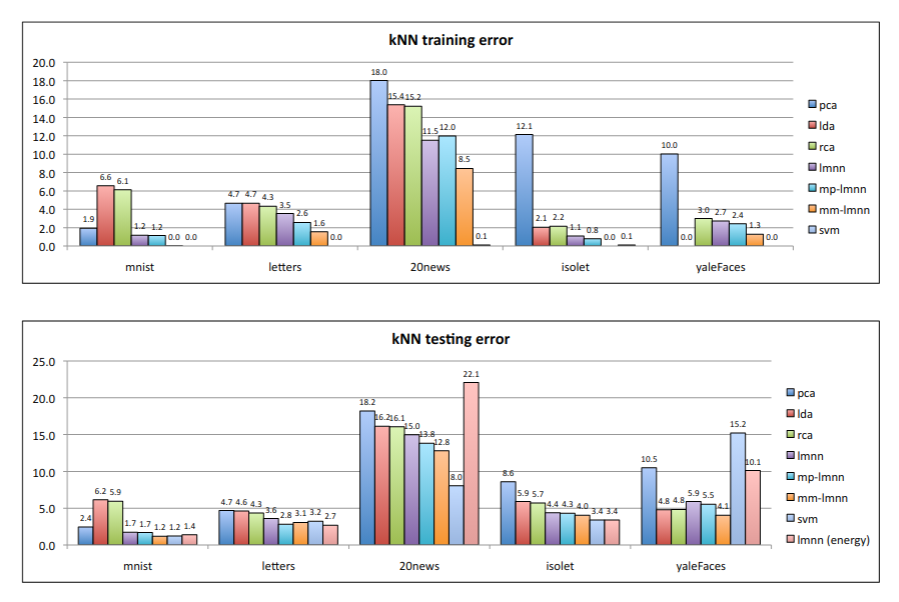
\includegraphics[width=0.7\textwidth]{res/result1.png}
    \caption{Result1}
    \label{fig:result1}
    \end{figure}
\end{frame}

\begin{frame}
    \frametitle{Face Recognition Results}
    \begin{figure}
    \centering
    
\includegraphics[width=0.6\textwidth]{res/result2.png}
    \caption{Test images from the Olivetti face recognition data set (top row). The middle row shows images from the same class that were among the 3-NN under the learned Mahalanobis metric (after training) but not among the original 3-NN under the Euclidean metric (before training). The bottom row shows impostors under the Euclidean metric that were no longer inside the local neighborhoods under the Mahalanobis metric.}
    \label{fig:result2}
    \end{figure}
\end{frame}


\begin{frame}
    \frametitle{Face Recognition Results}
        \begin{itemize}
            \item \textbf{Olivetti Face Dataset}
            \begin{itemize}
                \item 400 grayscale images of 40 subjects (10 poses/subject).
                \item Downsampled to 38×31 pixels, projected to 200 - eigenface subspace by PCA.
                \item 7 - train, 3 - test images per subject. LMNN improved accuracy, altered $k = 3$ NN.
            \end{itemize}
            \item \textbf{(Extended) Yale Face Dataset}
            \begin{itemize}
                \item 2414 frontal images of 38 subjects under extreme illumination.
                \item Pre - processed: downsampled, projected to 200 PCs, discarded 1st 5 eigenvectors.
                \item Results from 10 runs of 70/30 splits. LMNN outperformed Euclidean and SVMs.
            \end{itemize}
        \end{itemize}
\end{frame}

\begin{frame}
    \frametitle{Spoken Letter Recognition Results}
        \begin{itemize}
            \item \textbf{Isolet Dataset}
            \begin{itemize}
                \item From UCI Machine Learning Repository, has 6238 examples for 26 letter classes.
                \item Original dimension: 617. Projected onto 172 principal components (covering $95\%$ variance).
            \end{itemize}
            \item \textbf{Experimental Results}
            \begin{itemize}
                \item Dietterich and Bakiri achieved test error rates of $4.2\%$ $(26 - output units)$ and $3.3\%$ $ (30 - bit error - correcting code) $ using nonlinear backpropagation networks.
                \item LMNN with energy - based classification obtained a $3.4\%$ test error rate.
            \end{itemize}
            \item \textbf{Result Analysis}
            \begin{itemize}
                \item LMNN is an effective method for spoken letter recognition.
                \item Although not surpassing the best results, it shows potential in complex speech data classification.
            \end{itemize}
        \end{itemize}
    \end{frame}

\begin{frame}
    \frametitle{Letter Recognition Results}
        \begin{itemize}
            \item \textbf{Dataset Description}
            \begin{itemize}
                \item Taken from UCI Machine Learning Repository.
                \item Contains randomly distorted images of 26 English letters in 20 fonts.
                \item Features include 16 attributes like height, width, and axis correlations.
            \end{itemize}
            \item \textbf{Experimental Results}
            \begin{itemize}
                \item LMNN with energy - based classification significantly outperformed other variants of kNN classification on this dataset.
            \end{itemize}
            \item \textbf{Advantage Analysis}
            \begin{itemize}
                \item LMNN learns the Mahalanobis distance metric, effectively capturing complex data relationships.
                \item Its loss function design makes similar samples cluster closely and different - class samples separate well, enhancing adaptability and accuracy in letter recognition.
            \end{itemize}
        \end{itemize}
    \end{frame}

\begin{frame}
    \frametitle{Letter Recognition Results}
    \begin{figure}
    \centering
    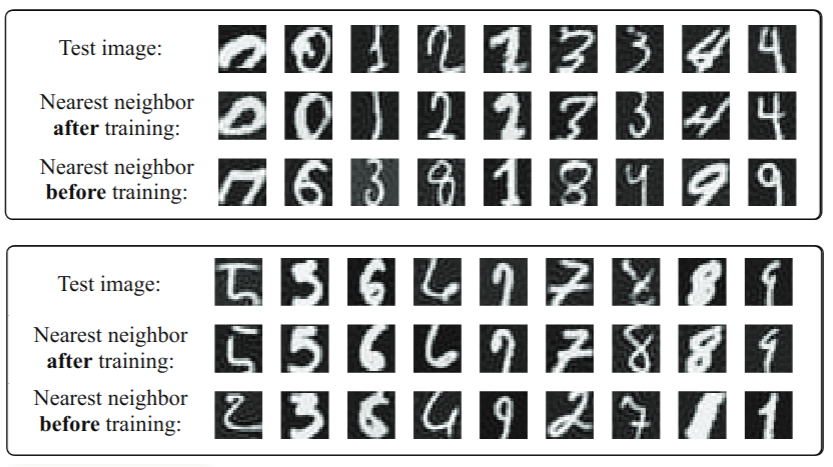
\includegraphics[width=0.7\textwidth]{res/result3.png}
    \caption{Images from the $MNIST$ data set, along with nearest neighbors before and after training.}
    \label{fig:result3}
    \end{figure}
\end{frame}
    
\begin{frame}
    \frametitle{Text Categorization Results}
        \begin{itemize}
            \item \textbf{Dataset}
            \begin{itemize}
                \item 20 - newsgroups: 18828 articles from 20 newsgroups.
                \item Tokenized, represented by 20,000 - word vectors, reduced to 200 PCs.
            \end{itemize}
            \item \textbf{Results}
            \begin{itemize}
                \item LMNN improved over kNN with Euclidean/PCA. Error rate: $14.98\%$ vs $48.57\%/18.22\%$.
                \item But multi - class SVM was better ($8.0\%$ error with linear kernel, 20,000D input).
            \end{itemize}
            \item \textbf{Analysis}
            \begin{itemize}
                \item LMNN used data features, but SVM was more effective for high - D text.
                \item Future research could optimize LMNN for text, e.g., new distance metrics.
            \end{itemize}
        \end{itemize}
    \end{frame}

\begin{frame}
    \frametitle{Handwritten Digit Recognition Results}
        \begin{itemize}
            \item \textbf{Dataset Description}
            \begin{itemize}
                \item The MNIST dataset of handwritten digits is widely benchmarked.
                \item Original $28\times28$ grayscale images were deskewed and projected onto 164 principal components (capturing 95\% variance).
            \end{itemize}
            \item \textbf{Experimental Results}
            \begin{itemize}
                \item Energy - based LMNN classification achieved a 1.4\% test error rate, cutting the baseline kNN error rate by over one - third.
                \item Compared with other benchmarks (no extra prior knowledge), multi - layer neural nets had a 1.6% error rate, and SVMs had a 1.2% error rate.
                \item The error rate of LMNN could be further reduced by learning different distance metrics for each digit class.
            \end{itemize}
            \item \textbf{Experimental Results}
            \begin{itemize}
                \item LMNN showed good performance on the MNIST dataset, improving the accuracy of handwritten digit recognition.
                \item Although there is still a gap compared with SVMs, it is close to the performance of multi - layer neural nets.
                \item Learning different distance metrics for each digit class can further improve the classification accuracy, providing a valuable direction for future research.
            \end{itemize}
        \end{itemize}
\end{frame}

\begin{frame}
    \frametitle{Handwritten Digit Recognition Results}
        \begin{itemize}
            \item \textbf{Dataset Description}
            \begin{itemize}
                \item MNIST: widely used for handwritten digit recognition.
                \item Images deskewed, projected to 164 PCs ($95\%$ variance).
            \end{itemize}
            \item \textbf{Experimental Results}
            \begin{itemize}
                \item Energy - based LMNN: $1.4\%$ test error, cut kNN error by over 1/3.
                \item Compared: multi - layer neural nets $(1.6\%)$, SVMs $(1.2\%)$.
                \item LMNN error can be further reduced with per - class metrics.
            \end{itemize}
            \item \textbf{Experimental Results}
            \begin{itemize}
                \item LMNN performed well, close to multi - layer neural nets.
                \item Per - class metrics offer potential for further improvement.
            \end{itemize}
        \end{itemize}
    \end{frame}
\begin{frame}
    \frametitle{Handwritten Digit Recognition Results}
    \begin{figure}
    \centering
    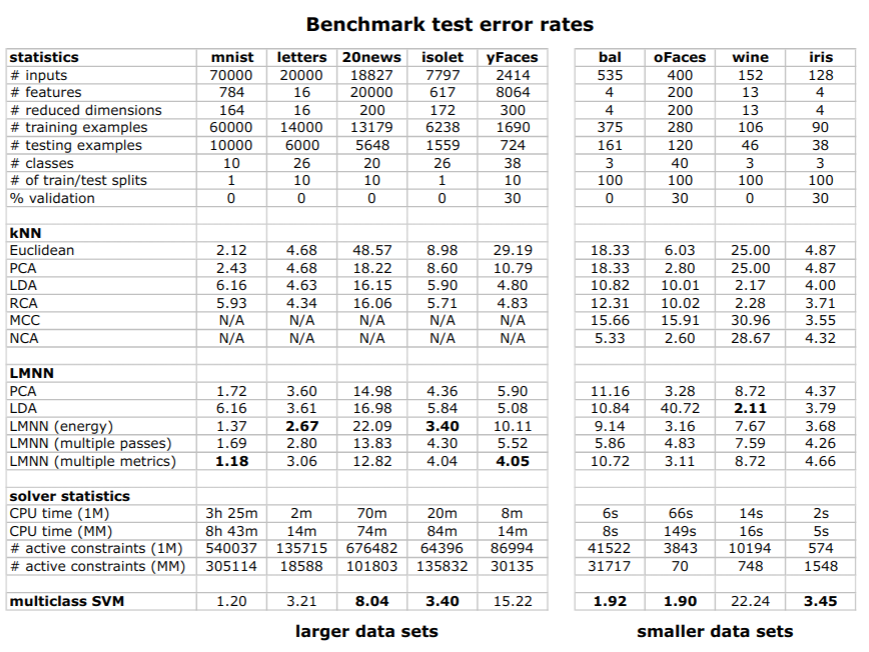
\includegraphics[width=0.38\textwidth]{res/result_table.png}
    \caption{Results and statistics of all experiments are presented. Datasets are ordered from largest to smallest. The table lists data stats and error rates of various LMNN training (single-pass, multi-pass, multi-metric), testing (kNN, energy-based), and preprocessing (PCA, LDA) methods. Results of RCA, NCA, and SVMs are included for comparison.}
    \label{fig:result_table}
    \end{figure}
\end{frame}

\begin{frame}
    \frametitle{Handwritten Digit Recognition Results}
    \begin{figure}
        \centering
        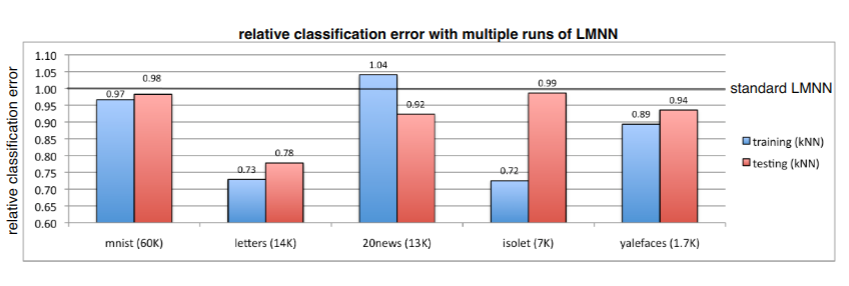
\includegraphics[width=0.7\textwidth]{res/result5.png}
        \caption{The relative change of the $3-NN$ classification error after multiple runs of LMNN over a
        single run of LMNN.}
        \label{fig:result5}
    \end{figure}
\end{frame}



\section{References}
\begin{frame}{References}
    \begin{thebibliography}{99}
    \bibitem{weinberger2009} Kilian Q. Weinberger, Lawrence K. Saul,
    "Distance Metric Learning for Large Margin Nearest Neighbor Classification",
    Journal of Machine Learning Research 10 (2009) 207 - 244
    \bibitem{cover1967} T. Cover, P. Hart,
    "Nearest neighbor pattern classification",
    IEEE Transactions in Information Theory, IT - 13, 21 - 27 (1967)
    \bibitem{belongie2002} S. Belongie, J. Malik, J. Puzicha,
    "Shape matching and object recognition using shape contexts",
    IEEE Transactions on Pattern Analysis and Machine Intelligence, 24(4), 509 - 522 (2002)
    \bibitem{simard1993} P. Y. Simard, Y. LeCun, J. Decker,
    "Efficient pattern recognition using a new transformation distance",
    in Advances in Neural Information Processing Systems 6, 50 - 58 (1993)
    \end{thebibliography}
\end{frame}



\end{document}